\documentclass[msc,oneside]{ubcthesis}%msc, phd, masc, ma, or meng

% ================================================================================
% CHANGE THE FOLLOWING ACCORDING TO YOUR PROGRAM/THESIS
% ================================================================================
\institution{The University Of British Columbia}
\program{Computer Science}
\faculty{THE IRVING K. BARBER SCHOOL OF ARTS AND SCIENCES}
\institutionaddress{Okanagan}

% For an Honours thesis, use \documentclasss[msc,oneside]{ubcthesis} above and
% uncomment and modify the next line:
\degreetitle{B.Sc. Computer Science Honours}

\title{The Source}
%\subtitle{With a Subtitle}
\author{Raffi Kudlac} % The name needs to be exactly the same as on the diploma i.e. (Name from SISC)
\copyrightyear{2015}
\submitdate{April 2015} % date of approved thesis
%\program{Interdisciplinary Studies - Optimization}%or Mathematics, or Interdisciplinary Studies
%\previousdegree{B.Sc. Hons., The University of British Columbia, 2008}
%\previousdegree{M.Sc., The University of British Columbia, 2010}

% ================================================================================


\usepackage{ubcostyle} %loads packages


% ===================================================================
% CHANGE THE FOLLOWING COMMANDS ACCORDING TO YOUR NEEDS
% ===================================================================
\newcommand{\R}{\mathbb{R}}   %real number
\newcommand{\Z}{\mathbb{Z}}   %integers
\newcommand{\C}{\mathbb{C}}   %complex numbers

\newcommand{\dom}{\operatorname{dom}}
\providecommand{\TT}[1]{\Theta\left(#1\right)} % big-Theta
\providecommand{\OO}[1]{\mathcal{O}\left(#1\right)} % big-Oh
% ===================================================================

%Uncomment the next line if there are more than one appendix
%\renewcommand*\appendixname{Appendices}


\begin{document}

% This starts numbering in Roman numerals as required for the thesis
% style.
\frontmatter                    % Mandatory

% The order of the following components should be preserved.  The order
% listed here is the order currently required by FoGS.
\maketitle                      % Mandatory

\newpage
\phantomsection \label{tableofcontent}%set anchor at right location
\addcontentsline{toc}{chapter}{\contentsname}
\tableofcontents                % Mandatory: generate toc
\newpage 
\phantomsection \label{listoftab}%set anchor at right location
\addcontentsline{toc}{chapter}{\listtablename}
\listoftables                   % Mandatory if thesis has tables
\newpage
\phantomsection \label{listoffig}%set anchor at right location
\addcontentsline{toc}{chapter}{\listfigurename}
\listoffigures                  % Mandatory if thesis has figures

% Any other unusual prefactory material should come here before the
% main body.

% Now regular page numbering begins.
\mainmatter

% Parts are the largest structural units, but are optional.
%\part{Thesis}

% Chapters are the next main unit.
\chapter{Introduction}
	“The Source” is an interactive simulation model where the user is charged with the task of providing 
energy to a growing population. The purpose of the simulation is to show the benefits and detriments of 
each type of energy source. Although the game targets young adults, primarily around high school and 
College/university students; anyone can play and and have a learning experience. Two intended outcomes of 
the simulation are to demonstrate the ratio of energy output to energy source type, and show the inner 
workings of each. A third outcome of the simulation is show that each type of energy works in the same way 
at its most basic level, with the exception of solar power converting kinetic energy into electrical energy.
\bigskip

The user will accomplish the task of providing energy by choosing to invest in different types of energy. 
The energy types that are at the users' disposal are solar, wind, hydro, coal, oil, gas and nuclear. Users 
can choose to build any of these power plants, but each type has consequences that others may not have. For 
example, if a user decided to build a power plant that ran off of coal, environmentalists would be 
displeased because the burning of coal introduces pollutants into the atmosphere. As well as considering 
the consequences of their actions, the users must also consider what fuels each power plant and how long 
each power plant can be sustained for. Fossil fuels and nuclear power are not infinite; the user must find 
resources to fuel these power plants. Users can choose to invest in renewable resources such as solar, wind 
and hydro, but the problem the user encounters with these types of resources is that they don't output as 
much energy as fossil fuels. The users' main objective is to survive for as long as possible and to beat 
their previous time. 

\chapter{Energy Today}
  In our society today almost all our energy that runs our homes and businesses is created in the same way 
It could be argued that, Micheal Faraday, the inventor of the concept of the generator had the biggest 
effect on the development of our society. In the early 1800's Micheal discovered that a magnet traveling 
through a coiled wire could generate a current and that once a current was generated it could be redirected 
to wherever it was needed. This concept is at the core of all our power generation.

\section{Generators}
  
  All generators operate in the same way of transferring kinetic energy into electrical energy. Some do 
  this buy having a stationary coil and moving a magnet through the coil as shown below or some have a 
  stationary magnet and move a coil through the magnetic field created by the magnet. It doesn't matter 
  which method is used, the same rules of physics are being applied and both ways achieve the result of a 
  flowing current. The faster the movement of the coil or magnet the more current that will be generated. 
  The more current that is generated to power there is to use. Generators have a couple more components to 
  them, gas chambers, rotating pistons ect.. these are all just tools used to convert the potential energy 
  of the power sourse into kinetic energy and finally into the desired electrical energy. This is at the 
  heart of all major production methods of power 
  as discussed below. 

  \begin{figure}[hbt]{\label{Induction} }
  \begin{center}
    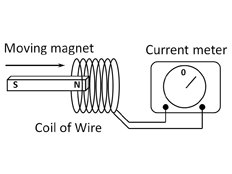
\includegraphics[width=0.3\textwidth]{Induction}
    \caption[Generator Mechanics]{Generator Mechanics}  
  \end{center}
\end{figure}

\newpage
  \section{Fossil Fuels}

  All Fossil fuel plants work in the same way, they burn a substance to heat water, that is turned into 
  steam that is then fed to flow past a turbine. The steam pushes the turbine which is connected to a 
  generator. This feeds kinetic energy to the generator which then turns the energy into electrical energy 
  for people to use.

Fossil fuel plants only differ in the substance that they burn, and some different protocols and buildings 
to handle the substances but the process is the same for all. Once the substance is burned the heat is 
transferred into water. In order to obtain as much energy as possible the water is kept under pressure 
making it able to be heated to temperatures much higher then $100^\circ$ C. Once the water is at a 
desired temperature it is fed through a series of pipes where it enters another chamber. In this chamber 
the water leaves the pipes at extraordinary speeds and instantly turned into steam as the pressure keeping 
the water in liquid form is being released. The fast moving steam pushes against a turbine causing it to 
move. In turn components in the generator are being turned and a current in generated. This is shown in figure \ref{FossilFuelCycle} which specifically shows the process of a coal power plant. 

   \begin{figure}[hbt] \label{FossilFuelCycle} 
  \centering    
    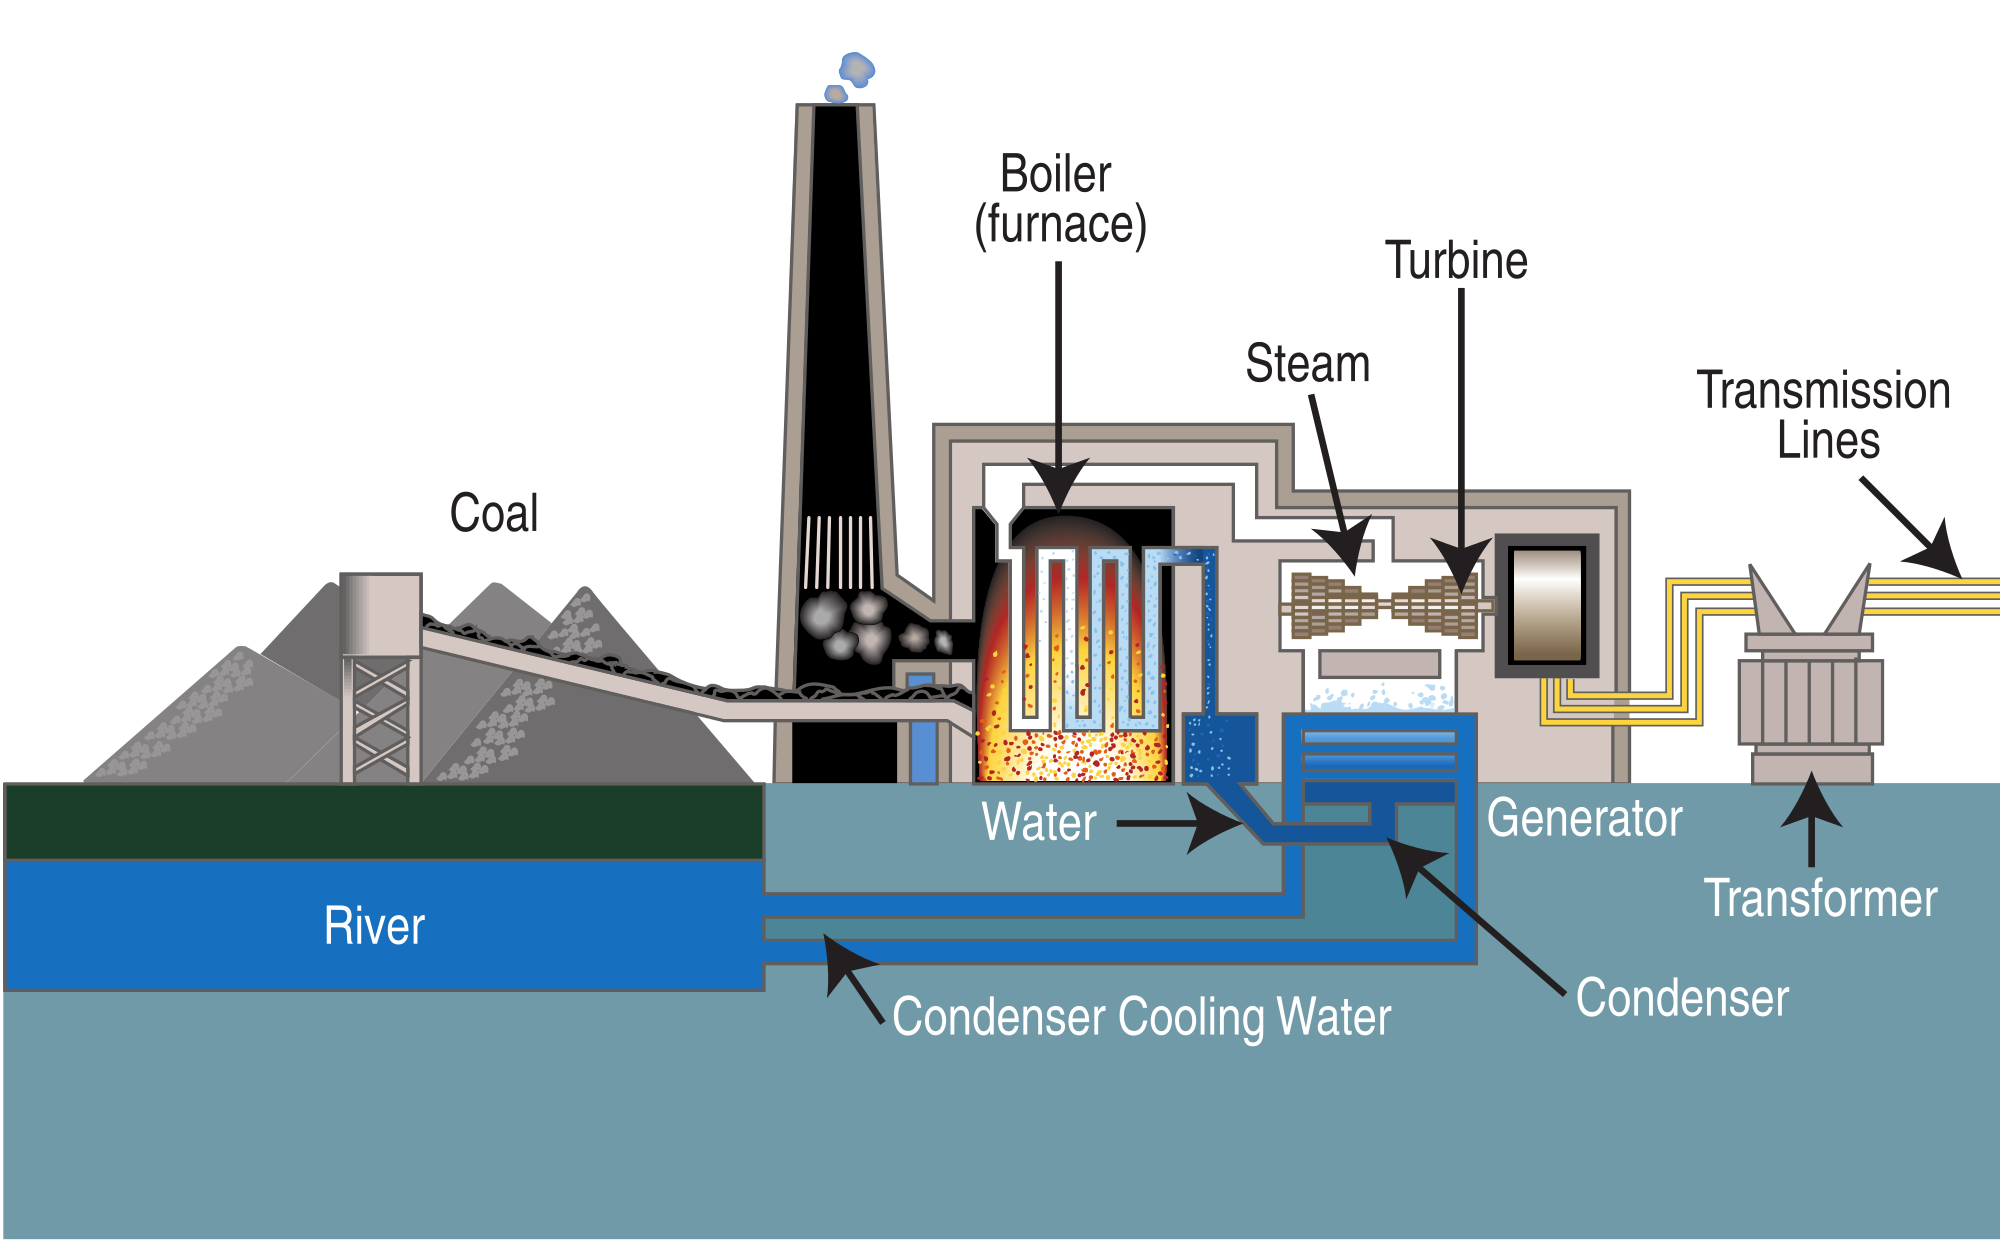
\includegraphics[width=1\textwidth]{fossil_fuel}
    \caption[Fossil Fuel Cycle]{Fossil Fuel Cycle}  
    
\end{figure}

\newpage

In order to save water the steam is collected and condensed back into water to be used again. Plants are 
usually built around a water source as water needs to switched out at times to cool components of the plant 
and since plants use water to function it convientient to have a water source close by.
 When water gets cycled out of the plant and back into the water source it is warm and can have negative 
 effects on wildlife. Imagine if someone cranked the heating in your house to $40^\circ$ C, how would you 
 like it?

Fossil fuel power plant generally produce large amounts of power and the price of fossil fuels is generally 
cheap but they have huge environmental consequences such as carbon dioxide. Fossil fuel plants also run on 
a limited resource and once the resource is depleted they will be useless.

 \section{Nuclear Power}

 Nuclear power,  maybe the most desired power source on the planet, is capable of producing tremendous 
 amounts of power for doing little work. All nuclear power plants today run off of fission, the process of 
 breaking up atoms into smaller ones and the magical element that nuclear plants run off of is Uranium. 
 Uranium has nice properties for being broken apart, one being that large amounts of energy are released 
 when fission is performed on it and this energy is given off in the form of heat. Just like fossil fuel 
 power plants, nuclear power plants operate by taking this heat, heating water into steam, using the steam 
 to turn a turbine and then the turbine turns a generator.

Of course the process of getting the heat is dramatically different. In the reactor of a nuclear power 
plant there are uranium rods, these fuel the plant. The rods are bombarded with nuclei that break apart the 
uranium when they collide. Essentially it's like breaking when playing pool. The cue ball is the nuclei and 
the triangle of pool balls is the uranium atom. Instead of sound being released when a collision occurs, 
heat gets released. The uranium rods are surrounded by water and this water absorbs the heat from the 
fission reaction. Just like in fossil fuel power plants the water is kept under pressure so that it can be 
heated to higher temperatures. Because this water is in direct contact with the radioactive core it is not 
turned into steam and is instead sent through a series of pipes away from the reactor. This water never 
leaves the pipes but is used to heat more water, safe water, that has outside contact with the pipes. From 
here the process is the same as with fossil fuel power plants. This is shown in Figure \ref{nuclearCycle}.

\begin{figure}[hbt]\label{nuclearCycle}
  \begin{center}
    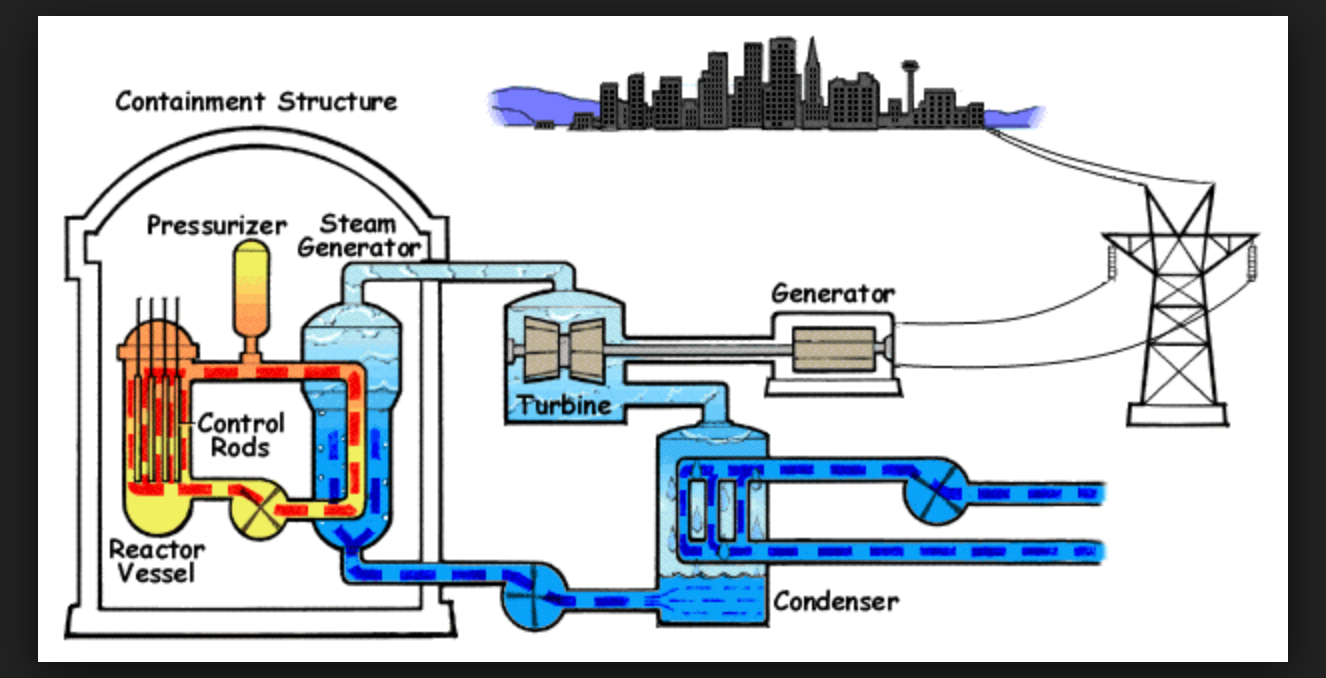
\includegraphics[width=1\textwidth]{nuclear}
    \caption[Nuclear Cycle]{Nuclear Cycle }
  \end{center}
\end{figure}

Nuclear power plants needs this extra step because the water that has direct contact with the core is 
radioactive and needs to be handled delicately. As a consequence it can't be in direct contact with other 
parts of the plant. Nuclear power plants have little waste compared to fossil fuel plants but they do 
produce radio active waste (left overs from the fission reaction) and it takes energy to mine the uranium, 
refine it and transport it to the plant.

Like fossil fuels, uranium is a element found in the earths crust and there is a finite amount of it. There 
is far more uranium then all the fossil fuels combined and we are using it up at a slower rate but one day 
we will run out and well weill have to find a new kind of power source for fission. 

\newpage
\section{Hydro Power}

Hydro power can arguably be the cleanest source of power due to the fact that it has almost no 
environmental effects once the plant is built. Like fossil fuels and nuclear power plants, hydro power 
plants works by turning a turbine that is connected to a generator to produce power but instead of using 
steam to push the turbine it uses liquid running water.

The rule of thumb for hydro power is the faster the water flows the more power you can generate. This 
creates a desire for big damns. The idea is that you damn a river causing the area above the damn 
to flood. The water is held at bay by the damn. Inside the damn there is a generator and turbines connected 
to it. The turbines are located in a shaft where water will flow. Once the shafts are open water runs 
through them powered by gravity and the water pressure from the lake. The bigger the damn, the bigger the 
lake, the more water pressure there is, the faster the flow of water, the more power generated. 
Figure \ref{hydroCycle} shows this process. Damns don't burn 
anything for fuel so there are no harmful environmental emissions once its running but damns usually 
require a giant areas of land to be destroyed. This wipes out any wildlife living there at the time and 
causes giant environmental shifts to wildlife. 

There are some rare cases such as Niagara falls where hydro generators can be placed beneath the falls and 
naturally falling water does the job with no assistance, so no damns need to be built. Finding a big enough 
waterfall that can generate enough power near a populated area is rare so this is not the usual option when 
creating a hydro electric damn. 

\begin{figure}[hbt]\label{hydroCycle}
  \begin{center}
    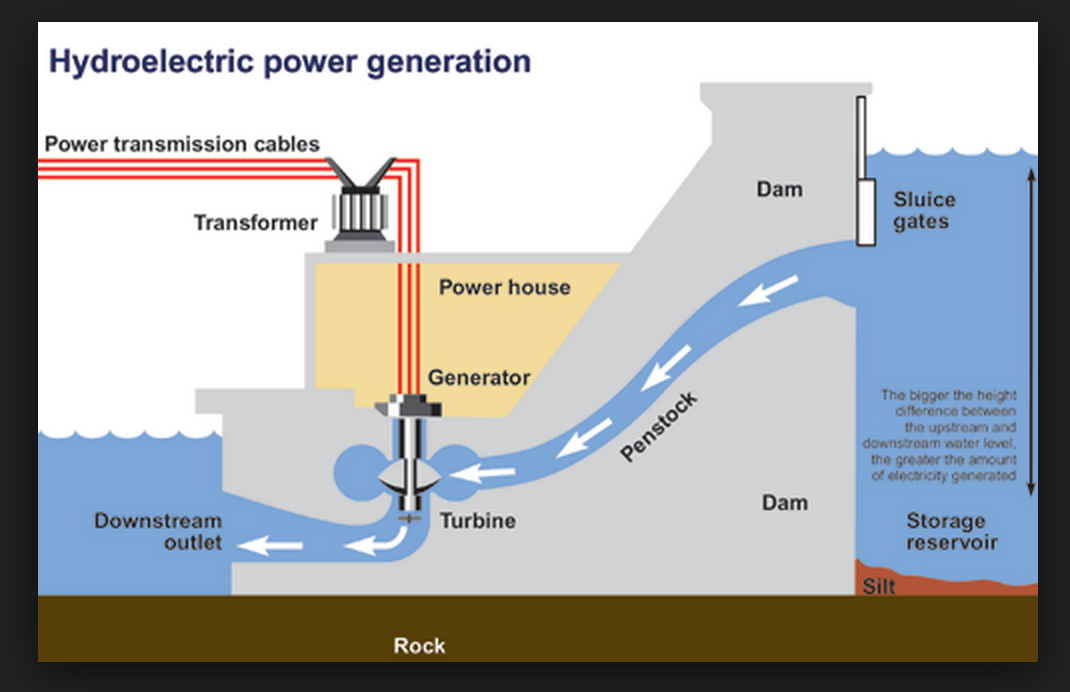
\includegraphics[width=1\textwidth]{hydro}
    \caption[Hydro Cycle]{Hydro Cycle }
  \end{center}
\end{figure}

\newpage

\section{Wind Power}

Wind power has maybe the least environmental impact out of all the power sources. They use wind currents to 
rotate giant blades that are in turn connected by a series of leavers and gears that are directly connected 
to the generator. Figure \ref{windmillWorkings} shows this process. The current is then fed down the shaft 
of the windmill and off to a population. Once constructed windmills essentially have no maintenance cost 
and are practically self sustaining except for breakdowns. 

Although windmills have minimal environmental effects they have drawbacks that they do not produce a lot of 
power and that they take up large amounts of space. Windmills kill a fair amount of birds per year and 
humans that live around them are no fan of the noise nor frequent shadows that they create. They are also 
costly to build and can only be placed in windy locations to make them worth building. 
\bigskip


\begin{figure}[hbt]\label{windmillWorkings}
  \begin{center}
    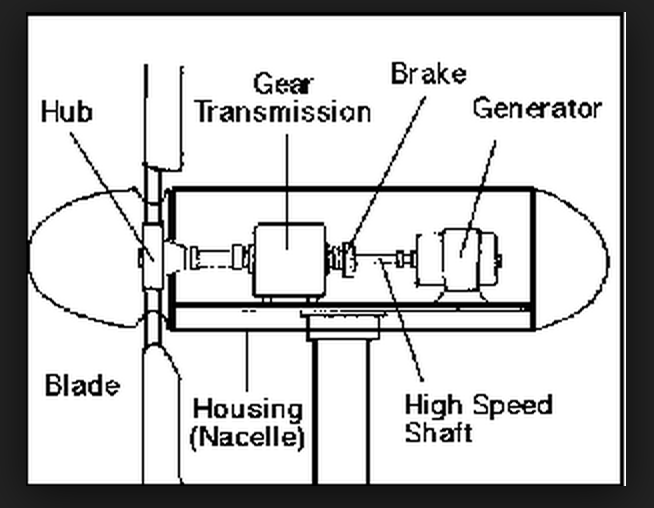
\includegraphics[width=1\textwidth]{windmill}
    \caption[Windmill Workings]{Windmill Workings }
  \end{center}
\end{figure}

\newpage

\section{Solar Power}
Solar power is the one power source that works completely different from all the others. Most objects when 
struct with light obsorb the incomming light rays and the energy gets converted into heat. Solar panels are made from a special substance, 
usually silicon that when struct with light react differently. When the electrons in solar panels are 
struct with light they get excited and they raise an energy level. When enough electrons are at high enough 
energy levels they become loose and are able to move around. Solar panels are specially built so that part of the panel holds a positive charge and the other part holds a negative charge. This makes the loose electrons, in the negative part of the panel want to move to the positive section. This forms a current in the cell and from here all we have to do is redirect the current to where ever we want it. Figure 
\ref{solarCell} shows this process. 

Although solar panels have barely no maintenance cost, fit nicely on rooftops and have hardly no 
environmental impacts they are the least efficient form of power, transforming  only about 20 percent of 
the sunlight that hits them into usable electricity. Solar panels are also expensive to build and in order 
to generate any significant amount of usable power from them for a mediocrely sized population, farms of 
solar panels need to be built and this takes up a huge amount of space.  Another giant draw back is that 
they only work during the day meaning another source of power is required for night time activities. 
\bigskip

\begin{figure}[hbt]\label{solarCell}
  \begin{center}
    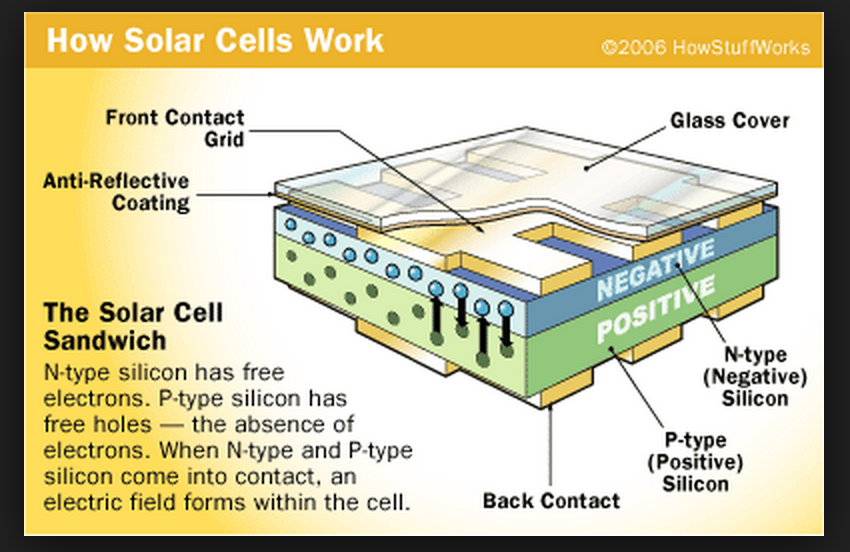
\includegraphics[width=1\textwidth]{solar}
    \caption[Solar Cell Workings]{ Solar Cell Workigns}
  \end{center}
\end{figure}

\newpage

\chapter{The Sourse}

The design of the system, as illustrated in figure 3.1 below, is straightforward. The user interacts with 
the system by purchasing power plants. This is done on a designated screen when there is land for the user 
to build on. Once the user has picked a type of power he/she must then provide the resources necessary for 
the power plant to function. The user can obtain fossil fuels by mining for them on the screen designated 
to represent the land that is currently available for the user to excavate. Once resources have been 
obtained and a power plant is built, energy can then be created and supplied to the population.
\bigskip

\begin{figure}[hbt]
  \begin{center}
    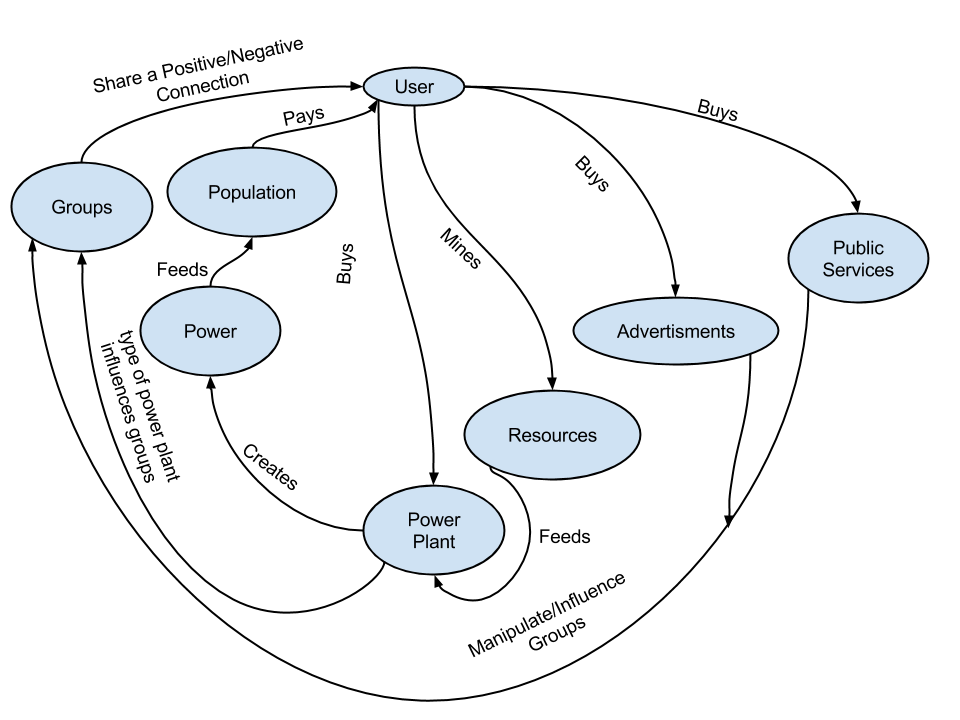
\includegraphics[width=0.9\textwidth]{DFDDiagram}
    \caption[Figure 1]{\label{DFD Diagram} }
  \end{center}
\end{figure}


Another option that the user has is that he/she can purchase advertisements or public services to help 
him/her flourish in the simulation. For example, a user could purchase an advertisement that educates the 
population to not waste power. This advertisement would reduce the usage of power and allow the user to 
more easily meet the demand. Users can also buy public services. An example would be a geologist that would 
survey the land and tell the user where to mine for a specific resource. Both of these purchases can 
influence groups within the game, such as environmentalists or public opinion. 
\bigskip


Users choices in the game affect groups as well, for example if a user invested in coal fueled power plants then the environmentalists group would not be displeased. Groups provide small perks or punishments to the user, usually in the form of grants or fines, which are dependent on the users play style and choices within the simulation. 


\section{Screen Layout}
“The Source” is composed of 8 different screen. The first five mentioned below are know as the five core screens. You can get to any of these screens from any other screen in the game. 
\bigskip

\noindent \large \textbf{ The Business Screen (one of the five core screens):} \newline
\indent In this screen the user is able to purchase advertisements and pubic services to help him/her 
progress through the simulation. Here the user is also able to see their progress throughout the game. The 
user will be able to see data like, money and energy made over time.  
\bigskip

\noindent The City Screen (one of the five core screens): \newline
\indent Here the user is able to see how the population is doing, the amount of power currently demanded and the amount supplied. This screens purpose is to purely display information.
\bigskip

\noindent The Power Plant Screen (one of the five core screens): \newline
\indent This screen, possibly the most education screen shows the workings of each type of energy as well as the inner workings of a generator. As well as seeing this information this screen allows the user to 
see specifics on the current power plants that he/she has built. Specifics being information such as 
amount of power produced, cost to maintain, resources required to maintain and more. 
\bigskip

\noindent The Land Screen (one of the five core screens): \newline
\indent From this screen the user can build power power plants that run off of fossil fuels and uranium. The user will have some designated land to start but he/she also has the option to buy more land to build 
on if the starting land is all used up.
\bigskip

\noindent The Resource Screen (one of the five core screens): \newline
\indent The purpose of this screen is to act like a map for the resources at the users disposal. From this 
screen the user can see all the resource that will be needed and the user can get at the three resource 
screens that will allow the user to extract the resources.
\bigskip

\noindent The Hydro Screen: \newline
\indent From here the user can view numerous rives that could be damned in order to generate power. Once a 
river is damned it will be shown on the screen. Rivers can only be damed once. 
\bigskip

\noindent Solar/wind Power Screen: \newline
\indent This screen shows land in the form of a grid that the user has at his/her to build windmills on or 
solar canals. Building will have a cost. Once something is built it can be dismantled to open the land 
to have something else built. 
\bigskip


\noindent The Fossil Fuels Screen: \newline
\indent Here land that the user can mine will be shown. This will be one large grid that will hold all the 
fossil fuels and uranium. The user can mine a section by selecting it and he or she will have a chance 
of discovering any one of the four resources. The resource discovered will go towards fueling the built 
power plants. Once a section is mined it can not be reused. 
\bigskip

\noindent The Static Screen: \newline
\indent The static screen is not really a screen at all but a combination of static images that remain on 
top of all other screens for the entire duration of the game. This serves as the means of navigation 	
between the five core screens. As well as displaying some information such as money and time. 
\bigskip

%Include citations in your thesis as you write:
%\cite{MR2848848,MR2461448,MR2834159,infconv,convmono,MR2668638,Bauschke:2007-PA02,proxbas}

%\section{Packages}
%There are several packages\ . So before you add a new package, check first if it is already included there.


%\section{Epigraph}
%If you want to add an epigraph to a chapter (epigraph in the sense of a literary inscription, not a function epigraph), you can use the command \texttt{epigraph} after the chapter. Check out the documentation of the \texttt{epigraph} package for more information.

% The following are examples of how to incorporate graphics into your thesis.

% \begin{figure}[ht]
%   \begin{center}
%     \includegraphics[width=0.4\textwidth]{figure}
%     \caption[Sample figure.]{\label{fig:happy} This is a sample figure
%       Note that we have
%       used the optional argument for the caption command so that only
%       a short version of this caption occurs in the list of figures.}
%   \end{center}
% \end{figure}

% \begin{figure}[ht]
%   \begin{center}
%     \includegraphics[width=0.4\textwidth]{figure}
%     \caption{\label{fig:happy2} This is the same sample figure with still
% 			a long caption but this time we did not use a short caption command
% 			in the table of figures.}
%   \end{center}
% \end{figure}

% You should really put text in between figures so LaTeX has more flexibility to place the figure at the appropriate location.



\chapter{Sample Content Using Mathematical Notations}

\section{Facts and theorems}
If we use a well established fact or theorem\ 

\begin{fact}\cite[Theorem~IV.2.4.2]{Hiriart-Urruty:1993-ConvexAnalysis}\label{def:marginalfunc}
Define the \emph{marginal function} $\gamma$ associated with $g:\R^n\times\R^m\rightarrow \R\cup
\{+\infty\}$ by $z\mapsto \gamma(z):=\inf_x
g(x,z)$. If $g$ is a proper convex function and is bounded below on the set  $\R^n \times \{z\}$ for all $z$, then $\gamma$ is convex.
\end{fact}

\section{Propositions and lemmas}
Here is a lemma followed by its proof.
\[
D =\left\{ (x,\lambda)\in \R^d \times \R^+ : \frac{x}{\lambda} \in C\right\}.
\]

\begin{lemma}
Assume $C$ is a nonempty closed convex set. Then the set $D$ is a nonempty closed convex cone.
\end{lemma}

\begin{proof}
The fact that $D$ is nonempty and closed follows from $C$ being non\-empty and closed. One can check directly that $D$ is a cone....

Hence $D$ is convex.
\end{proof}
Make sure that the qed symbol is always on the last line of the proof. If the last line is an equation, you can enforce the qed on the same line with the \texttt{qedhere} command.

For citations, please use BibTex. A sample article to verify formatting and style is \cite{Bauschke:2007-PA02}. Use the bibliography style \texttt{ubco}, which is basic \texttt{alphaurl} style with inline links enabled. Please compile multiple times when generating the references. The last entry in a reference are the back references to the pages with the citation. They need an additional compilation, once the bibtex entries are generated.

Note that the bibliography style is discipline dependent so feel free to use the style adopted by your discipline, for example siam for mathematics.

\chapter{Landscape Mode}
The landscape mode allows you to rotate a page through 90 degrees.  It
is generally not a good idea to make the chapter heading landscape,
but it can be useful for long tables etc.

\begin{landscape}
  This text should appear rotated, allowing for formatting of very
  wide tables etc.  Note that this might only work after you convert
  the \texttt{dvi} file to a postscript (\texttt{ps}) or \texttt{pdf}
  file using \texttt{dvips} or \texttt{dvipdf} etc.
\end{landscape}

\chapter{Conclusion}
Here comes the conclusion.
\begin{table}[tbph]
\centering
\caption{A publication quality table. Very very very very very very very very very very long title.
\label{table:food1}}
\begin{tabular}{@{}llr@{}} \toprule 
\multicolumn{2}{c}{Item} \\ \cmidrule(r){1-2} 
Animal & Description & Price (\$)\\ \midrule 
Gnat & per gram & 13.65 \\ 
& each & 0.01 \\ 
Gnu & stuffed & 92.50 \\ 
Emu & stuffed & 33.33 \\ 
Armadillo & frozen & 8.99 \\ \bottomrule 
\end{tabular}
\end{table}

\newpage
Your conclusion can go on for several pages.


% This file is setup to use a bibtex file sample.bib and uses the
% plain style.  Other styles may be used depending on the conventions
% of your field of study.
%
% Note: the bibliography must come before the appendices.


%change heading ``Chapter 5 Bibliography''->''Bibliography''
\newpage %newpage needed otherwise pagestyle applied to previous chapter. Does not actually create a new page
\pagestyle{fancy}\chead{Bibliography}\rhead{}\cfoot{}\rfoot{\thepage}

%Bibliography style is discipline dependent. Mathematic student can use e.g. SIAM
\bibliographystyle{ubco}
%\bibliographystyle{siam}
\bibliography{bibliography}%name of your .bib file

\newpage
\pagestyle{headings}
\addtocontents{toc}{%
\protect\renewcommand*\protect\cftchappresnum{\appendixname~}}

\appendix 
\addappheadtotoc %uses the current page number when it makes the entry in the ToC
\appendixpage 

\addtocontents{toc}{
\setlength{\cftbeforechapskip}{\cftbeforesecskip}
\setlength{\cftchapindent}{\cftsecindent}
\protect\renewcommand{\cftchapfont}{\cftsecfont}
\protect\renewcommand{\protect\cftchapdotsep}{\cftsecdotsep}
}


\chapter{Tables}
Here you can have additional tables. Table captions are always on top.

In order to use publication quality tables, one should use the guidelines in \cite{Fear:2005manual}. In short, do not use vertical rules or double rules, units in the column heading (not in the body of the table), precede decimals with a digit, and do not use ditto signs. Table \ref{table:food} is according to the guidelines. 

For tables, the caption goes on top, for figures, the caption goes on the bottom. If possible, always position tables and figures at the top of a page.\footnote{In this case, the chapter heading prevents the table from being at the top.} Use the option \verb|tbph| for the placement.

\begin{table}[tbph]
\centering
\caption{A publication quality table. Very very very very very very very very very very long title.
\label{table:food}}
\begin{tabular}{@{}llr@{}} \toprule 
\multicolumn{2}{c}{Item} \\ \cmidrule(r){1-2} 
Animal & Description & Price (\$)\\ \midrule 
Gnat & per gram & 13.65 \\ 
& each & 0.01 \\ 
Gnu & stuffed & 92.50 \\ 
Emu & stuffed & 33.33 \\ 
Armadillo & frozen & 8.99 \\ \bottomrule 
\end{tabular}
\end{table}

\newpage
And other table materials (I needed to generate two pages for that appendix to test the formatting of the table of content).

\begin{table}
\caption{Another table}
\end{table}

\begin{table}
\caption{Another table}
\end{table}
\begin{table}
\caption{Another table}
\end{table}
\begin{table}
\caption{Another table}
\end{table}
\begin{table}
\caption{Another table}
\end{table}

\begin{table}
\caption{Another table}
\end{table}
\begin{table}
\caption{Another table}
\end{table}
\begin{table}
\caption{Another table}
\end{table}
\begin{table}
\caption{Another table}
\end{table}
\begin{table}
\caption{Another table}
\end{table}

\chapter{Figures}
Here you can have additional figures. Figure captions are always at the bottom.

\newpage

And other additional figures (again I needed to generate two pages :-).
% Indices come here.


\end{document}
\endinput
